\section{Indgangsvinkel}
\label{DatabehandlingRIndgangsvinkel}
%
I dette afsnit analyseres resultaterne med udgangspunkt i de tre forskellige indgangsvinkler robotten havde til testpersonerne i testen og hvis testpersonerne selv henvendte sig. De forskellige indgangsvinkler fremgår af \autoref{tab:RDistance}, hvor antallet af testpersoner ligeledes er opgivet. 

Det undersøges, hvordan robottens indgangsvinkel for henvendelse påvirker de rejsendes oplevelse af robotten ved at undersøge, hvordan resultaterne ændrer sig afhængigt af de tre forskellige indgangsvinkler samt testpersonernes egen henvendelse. Det er et \textit{Between-subject} design, da hver testperson kun har oplevet robotten i én af indgangsvinklerne eller selv henvendt sig, og svaret ud fra dette.
%
\begin{table}[H]
\centering
\begin{tabular}{c|c}
Indgangsvinkel & Antal testpersoner \\ \hline
Venstre (1) & 4    \\ \hline
Forfra (2) & 18    \\ \hline
Højre (3) & 8     \\ \hline
TP henvender sig (4) & 13 \\
\end{tabular}
\caption{Oversigt over antallet af testpersoner (TP) til hver af de tre indgangsvinkler robotten havde samt hvis testpersonerne selv henvendte sig.}
\label{tab:RDirection}
\end{table}
\noindent
%
Ud fra \textit{Scree}-plottet på \autoref{fig:Direction-Scree} fremgår det, at cirka 60 \& af variansen kan forklares ud fra den første \textit{Principal Component} (PC) og 90 \% af variansen kan forklares ud fra to PCs, hvor PC2 bidrager med cirka 30 \%. Gøres der brug af alle tre PCs forklares 100 \% af variationen. 
%
\begin{figure}[H]
\centering
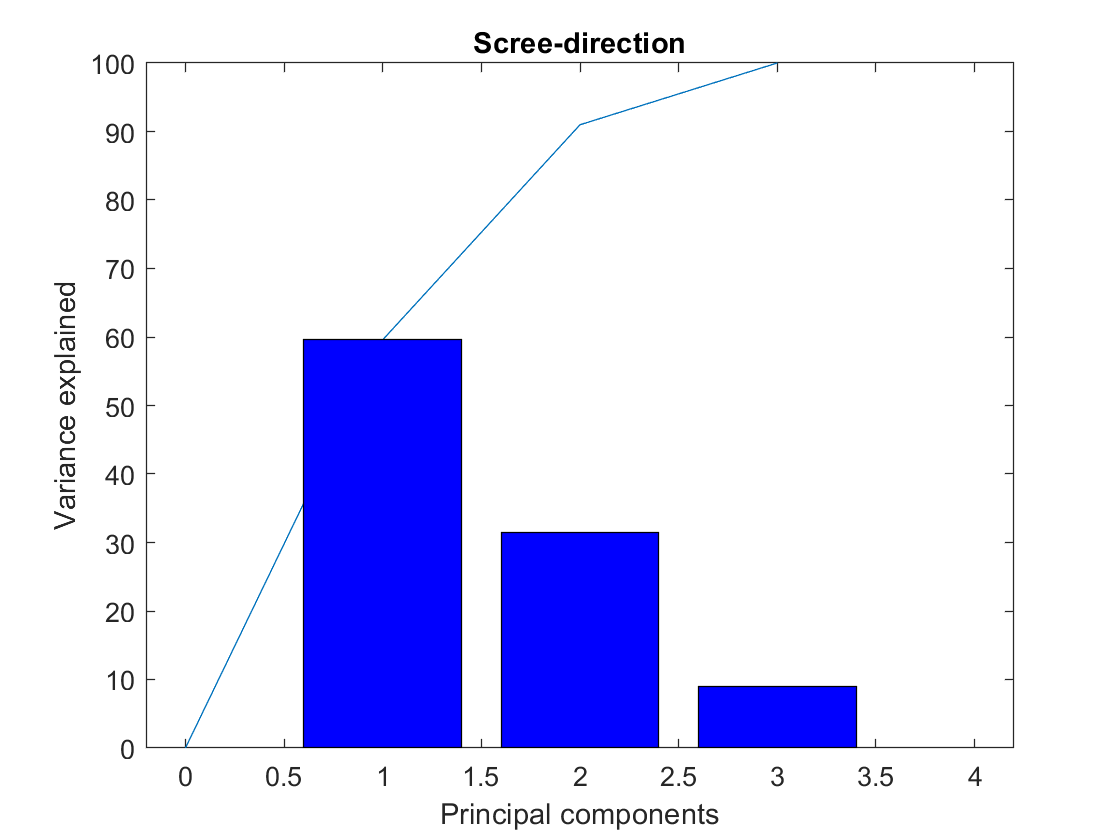
\includegraphics[width=\textwidth]{Figure/DatabehandlingSkalaer/PCAfigures/Direction-Scree.png}
\caption{\textit{Scree}-plot, hvorpå sammenhængen mellem antallet af \textit{Principal Components} og \textit{Variance Explained [\%]} fremgår.}
\label{fig:Direction-Scree}
\end{figure}
\noindent
% 
Ud fra \textit{Score}-plottet på \autoref{fig:Direction-Score} fremgår det, at der generelt er en del spredning mellem resultaterne ud fra de tre forskellige indgangsvinkler, hvilket foreskriver, at de tre indgangsvinkler ikke umiddelbart har ens karakteristikas. Dog ligger \textit{Kommer selv}, svarende til at testpersonerne selv henvendte sig til robotten, meget tæt på \textit{Forfra}, hvilket afspejler lignende karakteristikas for de to \textit{scores}. 
%
\begin{figure}[H]
\centering
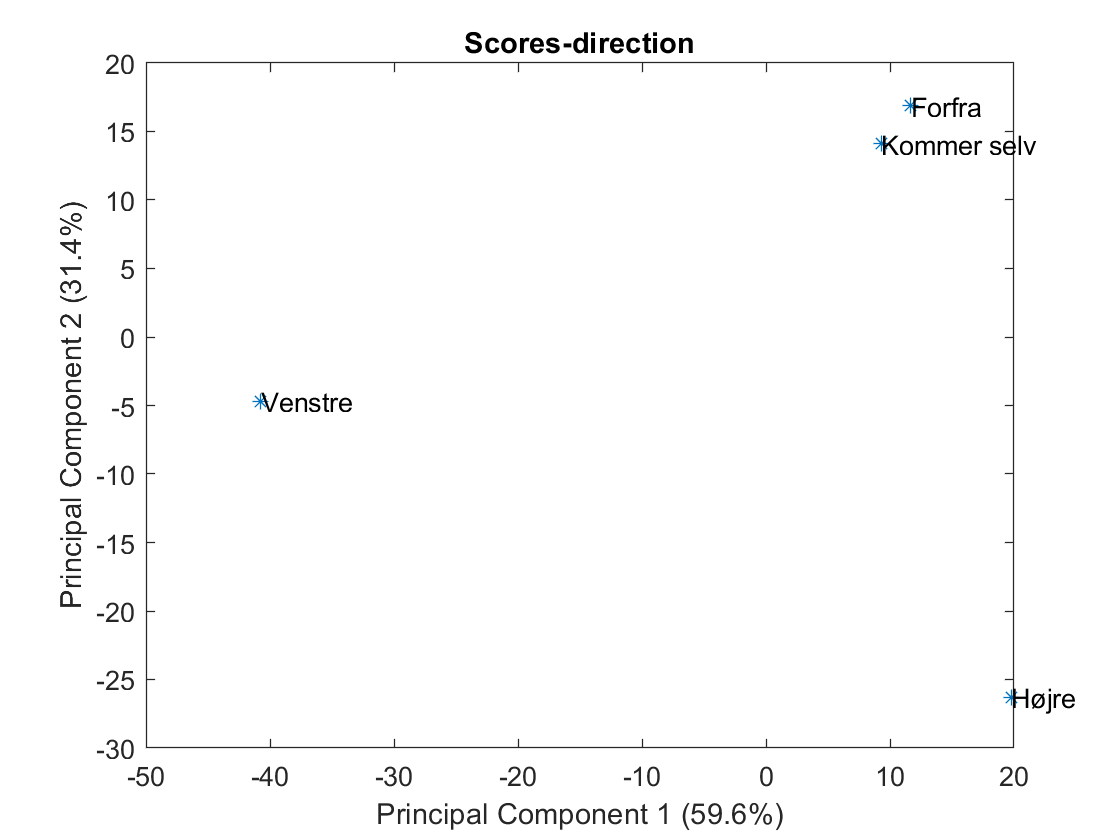
\includegraphics[width=\textwidth]{Figure/DatabehandlingSkalaer/PCAfigures/Direction-Scores}
\caption{\textit{Score}-plot for PC1 og PC2 i forhold til de tre indgangsvinkler robotten henvendte sig til testpersonerne med samt hvis testpersonerne selv henvendte sig.}
\label{fig:Direction-Score}
\end{figure}
\noindent
%
Ud fra \textit{Bi}-plottet på \autoref{fig:Direction-Biplot}, hvorpå \textit{loadings} og \textit{scores} for hver parameter er præsenteret, fremgår det at SQ10, vedrørende hvor tryg testpersonerne er ved robotten, forklare den største varians for PC1. For PC2 fremgår det, at både SQ1, vedrørende skærmens reaktion, SQ20, vedrørende hvor sej robotten opleves, samt SQ22, vedrørende hvor sjov robotten opleves, forklarer størstedelen af variansen. Da den forklaret varians fra SQ5, vedrørende robottens afstand, SQ6, vedrørende robottens hastighed, SQ7, vedrørende robottens højde, samt SQ16, vedrørende hvor irriterende robotten opleves, er relativt lille vil disse parametre ikke blive yderligere beskrevet, medmindre de indgår i en korrelation med en mere betydende parameter.  
%
\begin{figure}[H]
\centering
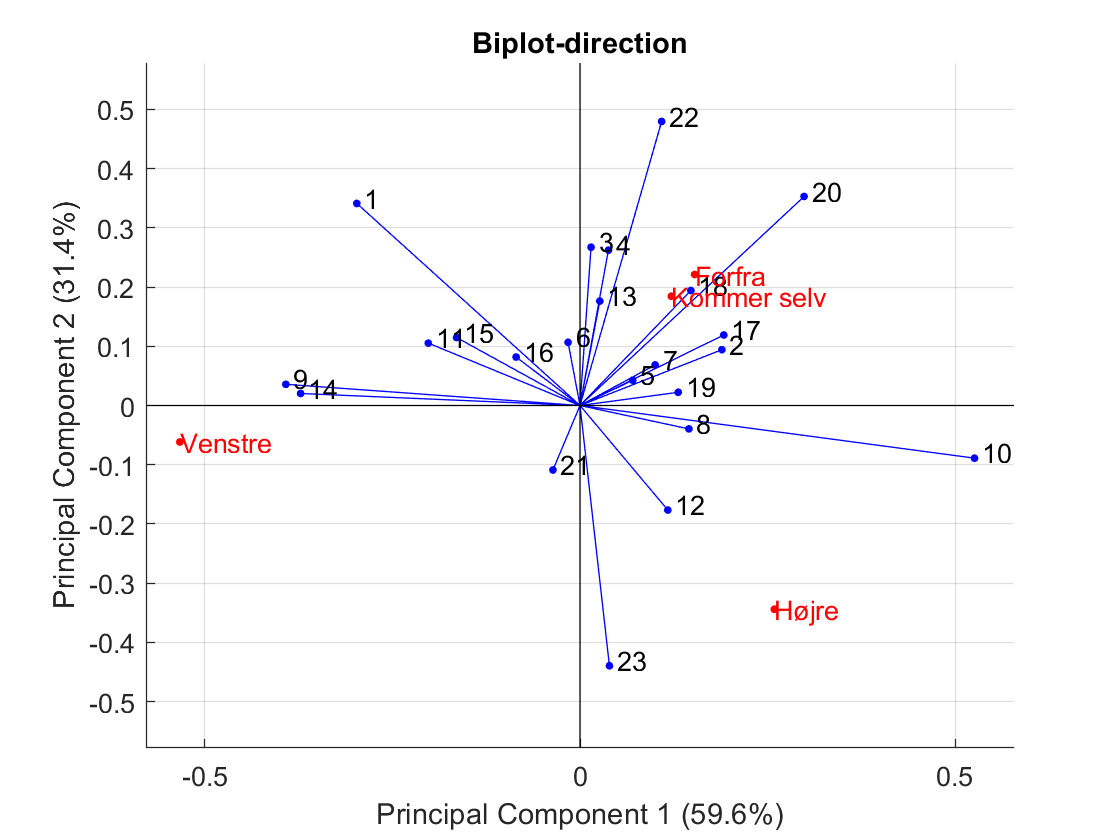
\includegraphics[width=\textwidth]{Figure/DatabehandlingSkalaer/PCAfigures/Direction-Biplot.png}
\caption{\textit{Bi}-plot med både \textit{loadings} (angivet med blå) og \textit{scores} (angivet med rød) fremgår i forhold til robottens indgangsvinkel.}
\label{fig:Direction-Biplot}
\end{figure}
\noindent
%
I forhold til korrelationen mellem parametrene, fremgår det at SQ18, vedrørede hvor spændende robotten opleves, og SQ20, vedrørende hvor sej robotten opleves, har en positiv korrelation. Den positive korrelation er gennemgående for flere af parametrene, SQ8, vedrørende hvorvidt testpersonerne føler, at robotten kan hjælpe dem, og SQ10, vedrørende hvor tryg testpersonerne er ved robotten, korrelerer ligeledes. Der forefindes en positiv korrelation mellem SQ9, vedrørende hvorvidt robotten stod i vejen, og SQ14, vedrørende hvor personlig testpersonerne oplevede robottens hjælp. SQ4, vedrørende robottens bevægelser, og SQ13, vedrørende hvorvidt testpersonerne følte, at robotten fulgte dem hen til det valgte sted, ligger oven på hinanden, hvorfor det vurderes at de korrelerer. Lignende gør sig gældende for SQ1 og SQ16, som også ligger tæt på \autoref{fig:Direction-Biplot}. Selvom SQ5 og SQ7 som tidligere nævnt forklare en meget lille del af variansen, så korrelerer de begge med SQ17, vedrørende hvor elegant robotten opleves.   

Udover de positive korrelationer forekommer der ligeledes negative korrelationer på \autoref{fig:Direction-Biplot}. Dette forekommer blandt andet mellem SQ1 og SQ12, vedrørende hvor godt testpersonerne kan lide at blive betjent af robotten. Den negative korrelation forekommer også mellem SQ21, vedrørende hvor anmassende robotten opleves, og SQ22, vedrørende hvor sjov robotten opleves. Den postive korrelation mellem SQ9 og SQ14 er negativ korrelerede med den postive korrelation mellem SQ8 og SQ10. Den sidste negative korrelation, der forefindes på \autoref{fig:Direction-Biplot}, er mellem SQ6, vedrørende robottens hastighed, og SQ23, vedrørende hvor menneskelig robotten opleves. \blankline
%
Hver \textit{loading} angiver hvor meget variation hver parameter bidrager med i forhold til den specifikke PC. I \autoref{tab:LoadingsIndgangsvinkel} fremgår samtlige \textit{loadings} for hver parameter til hver PC.  
%
\begin{table}[H]
\centering
\begin{tabular}{c|c|c|c}
    & PC1 (59.6\%)    & PC2 (31.4\%)    & PC3 (9\%)       \\ \hline
SQ1  & -0.2974         & 0.3412          & -0.2362         \\ \hline
SQ2  & 0.1890          & 0.0942          & -0.1122         \\ \hline
SQ3  & 0.0147          & 0.2673          & -0.0454         \\ \hline
SQ4  & 0.0379          & 0.2624          & 0.2993          \\ \hline
SQ5  & 0.0702          & 0.0427          & 0.0823          \\ \hline
SQ6  & -0.0159         & 0.1067          & 0.0165          \\ \hline
SQ7  & 0.1001          & 0.0686          & -0.0203         \\ \hline
SQ8  & 0.1451          & -0.0395         & 0.0291          \\ \hline
SQ9  & -0.3921         & 0.0358          & 0.0498          \\ \hline
SQ10 & \textbf{0.5258} & -0.0889         & -0.1395         \\ \hline
SQ11 & -0.2022         & 0.1053          & 0.3059          \\ \hline
SQ12 & 0.1170          & -0.1765         & 0.2387          \\ \hline
SQ13 & 0.0264          & 0.1764          & -0.4342         \\ \hline
SQ14 & -0.3724         & 0.0203          & 0.1812          \\ \hline
SQ15 & -0.1644         & 0.1147          & -0.2624         \\ \hline
SQ16 & -0.0851         & 0.0818          & 0.0851          \\ \hline
SQ17 & 0.1916          & 0.1191          & -0.1870         \\ \hline
SQ18 & 0.1478          & 0.1942          & 0.0192          \\ \hline
SQ19 & 0.1309          & 0.0223          & 0.2178          \\ \hline
SQ20 & 0.2987          & 0.3530          & \textbf{0.4448} \\ \hline
SQ21 & -0.0361         & -0.1089         & 0.2298          \\ \hline
SQ22 & 0.1088          & \textbf{0.4797} & -0.1187         \\ \hline
SQ23 & 0.0392          & -0.4395         & -0.1192        
\end{tabular}
\caption{Oversigt over \textit{loadings} til de tre PCs, for hver PC fremhæves den mest betydende parameter. \textit{SQ} angiver skala spørgsmålet.}
\label{tab:LoadingsIndgangsvinkel}
\end{table}
\noindent
%
Tages der derimod udgangspunkt i et tredimensionelt \textit{Bi}-plot, jævnfør \autoref{fig:Direction-3D}, fremgår det, at scoren for \textit{Forfra} og \textit{Kommer selv} ikke ligger lige så tæt på \autoref{fig:Direction-Biplot}, men derimod ligger \textit{Kommer selv} tættere på \textit{Højre}. Derudover er mange af de førnævnte positive korrelationer ikke længere korrelerede. På det tredimensionelle \textit{Bi}-plot, jævnfør \autoref{fig:Direction-3D}, fremgår det, at SQ1 og SQ16 i højere grad er ortogonale, hvilket gengiver at de ikke korrelerer. Lignende tendens forekommer ved SQ5 og SQ17, som er ortogonale fremfor korrelerede. I tillæg er SQ17 og SQ7 ikke længere placeret oven på hinanden, dog forekommer der en lille korrelation. Der forekommer ikke længere end positiv korrelation mellem SQ4 og SQ13 i det tredimensionelle \textit{Bi}-plot, jævnfør \autoref{fig:Direction-3D}, korrelationen er nærmere negativ. Korrelationen mellem SQ20 og SQ18 er heller ikke lige så høj, som tidligere, det tyder derimod på at SQ19 i højere grad korrelerer med SQ20. På \autoref{fig:Direction-Biplot} fremgår det at SQ21 er negativ korreleret med SQ22, dette er dog ikke tilfældet i \autoref{fig:Direction-3D}, hvor de to parametre i højere grad er ortogonale end negativ korrelerede. Dog forekommer der en negativ korrelation mellem SQ21 og SQ13.
%
\begin{figure}[H]
\centering
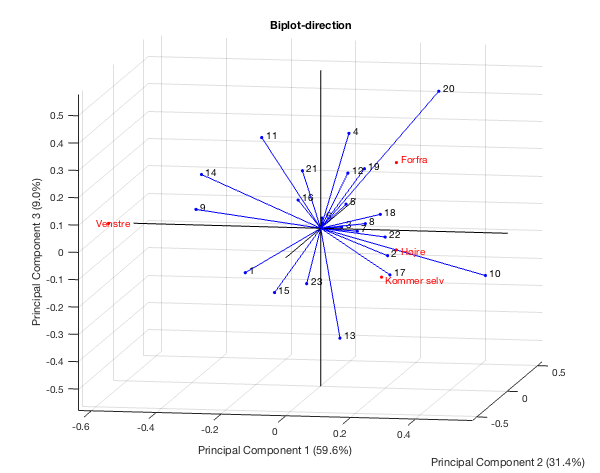
\includegraphics[width=\textwidth]{Figure/DatabehandlingSkalaer/PCAfigures/Direction-3D.png}
\caption{3D \textit{Bi}-plot med både \textit{loadings} (angivet med blå) og \textit{scores} (angivet med rød) fremgår i forhold til robottens indgangsvinkel eller hvis testpersonerne selv henvendte sig.}
\label{fig:Direction-3D}
\end{figure}
%


\subsection{Tendenser i forhold til robottens indgangsvinkel}
\label{DatabehandlingIndgangsvinkelTendenser}
%
Ligesom tilfældet med robottens afstand til testpersonerne, har det ikke været muligt at kontrollere indgangsvinklen, blandt andet fordi det afhænger af, hvor robotten er inden den henvender sig til en rejsende eller inden en rejsende henvender sig til den. Det har derfor ikke været muligt, at spore nogle tendenser, da der har været meget variation blandt besvarelserne.  

